\documentclass[a4paper,12pt]{article}
\usepackage{graphicx}
\usepackage{amsmath}
\usepackage{hyperref}
\usepackage{enumitem}
\usepackage{float}

\title{Events System Documentation}
\author{Bieber Fever}
\date{\today}

\begin{document}

\maketitle
\tableofcontents

\section{Introduction}
\label{sec:introduction}

\subsection{Vision and Objectives}
The vision for the Event System is to create a centralized, user-friendly platform that 
enhances employee engagement and fosters a vibrant organizational culture. By providing 
an efficient way to view, host, and RSVP to events, the system aims to improve communication, 
streamline event management, and encourage active participation in a variety of organizational 
activities. The primary objectives of the Event System are to:

\textbf{Increase Employee Engagement:} By making it easier for employees to discover and 
participate in events, the system aims to foster a more connected and engaged workforce.

\textbf{Simplify Event Management:} For hosts, the system provides tools to efficiently 
create, manage, and promote events, reducing the administrative burden and allowing for 
more focus on event quality and participation.

\textbf{Enhance Communication:} The system facilitates better communication about upcoming 
events through notifications and updates, ensuring that employees are always informed.

\textbf{Provide Insights:} Through analytics, the system offers valuable insights into 
employee participation and event success, enabling hosts and organizational leaders to 
make data-driven decisions for future events.

\subsection{Business Need}
In today's fast-paced work environment, maintaining high levels of employee engagement 
and morale is critical for organizational success. Traditional methods of promoting and 
managing events often fall short in terms of efficiency and reach. The need for a centralized 
platform is evident as it addresses several key challenges:

\textbf{Lack of Awareness:} Employees may miss out on events due to insufficient communication and visibility.

\textbf{Inefficient Management:} Hosts struggle with the logistical challenges of organizing and promoting events.

\textbf{Disconnected Workforce:} Without a cohesive system, opportunities for employee bonding and engagement are 
reduced, potentially impacting overall productivity and job satisfaction.

The Event System addresses these challenges by providing a streamlined, integrated solution that 
benefits both employees and hosts, ultimately contributing to a more dynamic and engaging workplace.

\subsection{Project Scope}
The scope of the project includes the development and implementation of an Event System with the following core functionalities:

\textbf{Event Creation and Management:} Hosts can create, edit, and delete events, providing 
detailed information and multimedia content to attract attendees.

\textbf{Event Details Viewing:} Employees can view comprehensive details about each event, 
including time, date, location, hosts, participants, and preparation instructions.

\textbf{Calendar View:} A calendar interface displays all upcoming events, allowing employees 
to easily plan their schedules.

\textbf{Filtering and Search:} Advanced filtering options and keyword search functionality 
help employees find events relevant to their interests and needs.

\textbf{RSVP Functionality:} Employees can RSVP to events, and hosts can track and manage attendance.

\textbf{Series Subscription:} Employees can subscribe to a series of events, ensuring they 
receive notifications for all related activities.

\textbf{Historical Events:} Employees can view a history of the events they have attended, 
along with any associated materials or recordings.

\textbf{Personal Information Management:} Employees can set and update personal preferences, 
such as dietary requirements, to streamline the RSVP process.

\textbf{Notifications:} Automated notifications keep employees informed about upcoming events 
and any changes or updates.

\textbf{User Management:} The system supports user registration, sign-in, and role-based 
permissions for managing event-related tasks.

\textbf{Analytics:} Providing insights into event participation and engagement trends to 
help hosts optimize future events.

\textbf{Event Registration with QR Code:} Streamlining event check-ins through scannable 
QR codes, enhancing the registration process.

By covering these functionalities, the Event System ensures a comprehensive, efficient, 
and user-friendly experience for all participants, significantly contributing to the overall 
goals of enhancing employee engagement and organizational cohesion.

\section{User Stories / User Characteristics}
\label{sec:user-stories}

\subsection{User Characteristics}

\subsubsection{Host}
Hosts are responsible for organizing, scheduling, and managing events within the organization. 
They create event listings, provide detailed descriptions, set dates, and handle logistics to 
ensure successful execution. Their primary goal is to promote employee bonding, engagement, and 
participation by curating events that are relevant and interesting to employees. They aim to foster 
a sense of community and enhance the workplace culture. Hosts are typically detail-oriented, possess 
strong organizational skills, and have a good understanding of the interests and needs of the employees. 
They should be adept at communication and marketing to effectively promote events. Hosts will require 
tools to manage event details, send invitations, track RSVPs, and gather feedback post-event. They 
will also need access to analytics to assess event success and employee engagement levels. 

\subsubsection{Employee}
Employees are the end-users of the Event System. They browse the events, RSVP to those they are 
interested in, and participate in the activities organized by the Hosts. They aim to find events 
that align with their interests, professional growth, or social engagement needs. Participation 
in these events is expected to enhance their sense of belonging and satisfaction within the organization. 
Employees vary widely in their interests and engagement levels. The system needs to be user-friendly to accommodate 
all employees, regardless of their technical proficiency. Employees will require a calendar view of upcoming events, 
search and filter options to find relevant events, RSVP capabilities, and reminders for events they plan to attend. 
They also need the option to provide feedback on events they attend.

\paragraph{Event Creation}

\begin{enumerate}
    \item As a Host, I want to create new events in the system so that employees can view and RSVP to them.
    \item As a Host, I want to edit event details so that I can update information if there are any changes.
    \item As a Host, I want to delete events that are no longer relevant so that the event list remains current.
\end{enumerate}

\paragraph{Event Details}

\begin{enumerate}
    \item As a Host, I want to add multimedia elements like images and videos to the event details so that the event 
    is more engaging and informative.
    \item As an Employee, I want to view detailed information about an event, including time, date, location, host, 
    participants, description, and preparation details, so that I can decide whether to attend.
    \item As an Employee, I want to see a map or directions to the event location so that I can easily find my way there.
\end{enumerate}

\paragraph{Calendar View}

\begin{enumerate}
    \item As a Host, I want to see a calendar view of all my events so that I can manage them efficiently.
    \item As an Employee, I want to see a calendar view of upcoming events so that I can easily plan my schedule.
    \item As an Employee, I want to add events to my personal calendar so that I can keep track of my commitments.
\end{enumerate}

\paragraph{Filtering}

\begin{enumerate}
    \item As an Employee, I want to filter events based on geolocation so that I can find events happening near me.
    \item As an Employee, I want to filter events based on social club so that I can find events related to my interests.
    \item As an Employee, I want to filter events using other criteria like date and category so that I can quickly 
    find relevant events.
    \item As an Employee, I want to filter events based on the type (e.g., in-person, virtual) so that I can find 
    events that suit my preference.
\end{enumerate}

\paragraph{Search}

\begin{enumerate}
    \item As a Host, I want to search for past events to review feedback and attendance data so that I can improve future events.
    \item As an Employee, I want to search for events using keywords so that I can find specific events quickly.
\end{enumerate}

\paragraph{RSVP}

\begin{enumerate}
    \item As a Host, I want to view the list of RSVPs for my events so that I can prepare accordingly.
    \item As an Employee, I want to RSVP to events so that the host knows I plan to attend.
    \item As an Employee, I want to change my RSVP status if my plans change so that the host has an accurate count of attendees.
\end{enumerate}

\paragraph{Series Subscription}

\begin{enumerate}
    \item As an Employee, I want to subscribe to a series of events so that I receive notifications for each event in the series.
    \item As an Employee, I want to manage my subscriptions to event series so that I can opt in or out as needed.
\end{enumerate}

\paragraph{Historical Events}

\begin{enumerate}
    \item As an Employee, I want to view a list of historical events I have attended so that I can keep track of my past engagements.
    \item As an Employee, I want to access materials or recordings from past events so that I can revisit the content.
\end{enumerate}

\paragraph{Personal Information}

\begin{enumerate}
    \item As a Host, I want to view and edit my profile information so that my contact details and preferences are up-to-date.
    \item As an Employee, I want to set my personal information, such as dietary requirements, in the system so that 
    I do not need to specify it each time I RSVP.
    \item As an Employee, I want to update my personal information easily so that my preferences are always current.
\end{enumerate}

\paragraph{Notifications}

\begin{enumerate}
    \item As a Host, I want to send notifications to employees about event updates or reminders to ensure maximum participation.
    \item As an Employee, I want to receive notifications about upcoming events so that I do not miss them.
\end{enumerate}

\paragraph{User Management}

\begin{enumerate}
    \item As a Host, I want to register an account on the system so that I can create events.
    \item As a Host, I want to sign in and verify my credentials so that I can securely access my account.
    \item As an Employee, I want to register an account on the system so that I can access event details and RSVP.
    \item As an Employee, I want to sign in and verify my credentials so that I can securely access my account.
\end{enumerate}

\paragraph{Analytics}

\begin{enumerate}
    \item As a Host, I want to view analytics and insights into employee participation in events so that 
    I can understand engagement levels and improve future events.
\end{enumerate}

\paragraph{Event Registration with QR Code}

\begin{enumerate}
    \item As a Host, I want to provide a scannable QR code for event registration so that attendance 
    tracking is streamlined and efficient.
    \item As an Employee, I want to easily indicate my attendance at events by scanning a QR code on 
    a signboard so that my presence is recorded without manual check-ins.
\end{enumerate}

\section{Functional Requirements}
\label{sec:functional-requirements}

\subsection{Requirements}

1. \textbf{Event Management}\\
    1.1. The system shall allow for the creation of new events.\\
    1.2. The system shall allow for the editing of existing event details.\\
    1.3. The system shall allow for the deletion of events.\\
    1.4. The system shall allow for the addition of multimedia elements (e.g., images, videos) to event descriptions.\\\\
2. \textbf{Event Details Viewing}\\
    2.1. The system shall allow for the viewing of detailed information about an event, including time, date, location, host, participants, description, and preparation details.\\
    2.2. The system shall provide a map or directions to the event location.\\\\
3. \textbf{Calendar View}\\
    3.1. The system shall provide a calendar view for managing events.\\
    3.2. The system shall provide a calendar view for seeing upcoming events.\\
    3.3. The system shall allow for the addition of events to personal calendars.\\\\
4. \textbf{Filtering and Search}\\
    4.1. The system shall allow for the filtering of events based on geolocation.\\
    4.2. The system shall allow for the filtering of events based on social clubs.\\
    4.3. The system shall allow for the filtering of events using criteria such as date, category, and type (e.g., in-person, virtual).\\
    4.4. The system shall allow for the searching of events using keywords.\\
    4.5. The system shall allow for the searching of past events to review feedback and attendance data.\\\\
5. \textbf{RSVP Functionality}\\
    5.1. The system shall allow for the RSVP to events.\\
    5.2. The system shall allow for the changing of RSVP status.\\
    5.3. The system shall allow for the viewing of the list of RSVPs for events.\\\\
6. \textbf{Series Subscription}\\
    6.1. The system shall allow for the subscription to a series of events.\\
    6.2. The system shall allow for the management of subscriptions to event series.\\\\
    feat(docs): requirements-
\section{Service Contracts}
\label{sec:service-contracts}

\section{Class Diagram}
\label{sec:class-diagram}
\label{sec:class-diagram}
\begin{figure}[H]
    \centering
    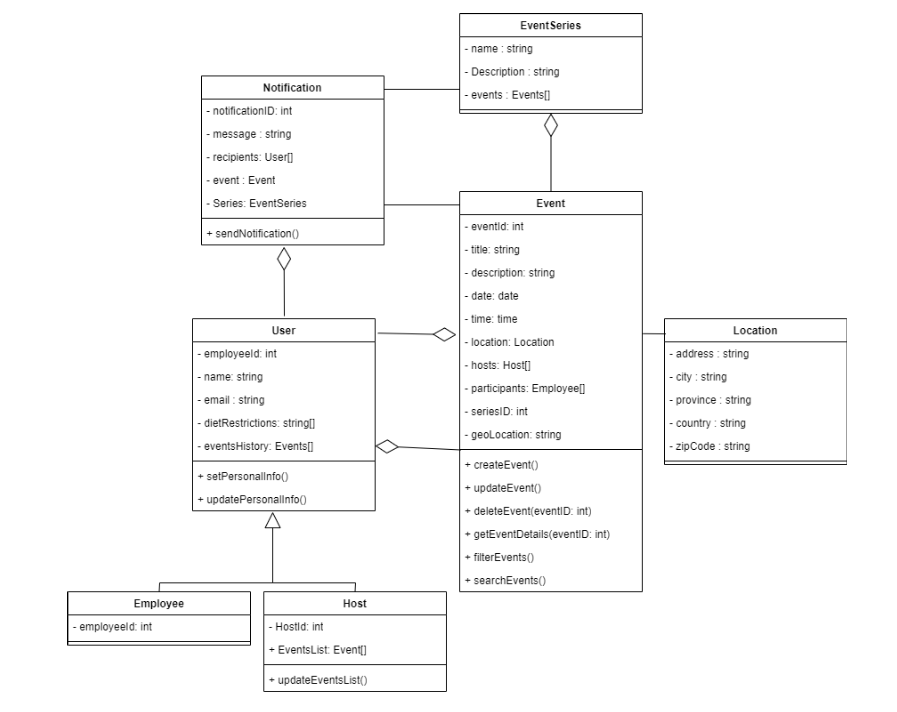
\includegraphics[width=\textwidth]{EventsClassDiagram.png}
    \caption{Class Diagram}
    \label{fig:class-diagram}
\end{figure}

\section{Architectural Requirements}
\label{sec:architectural-requirements}

\subsection{Quality Requirements}
\label{subsec:quality-requirements}

\subsection{Architectural Patterns}
\label{subsec:architectural-patterns}

\subsection{Design Patterns}
\label{subsec:design-patterns}

\subsection{Constraints}
\label{subsec:constraints}

\section{Technology Requirements}
\label{sec:technology-requirements}

\end{document}

